%% $RCSfile: proj_report_outline.tex,v $
%% $Revision: 1.2 $
%% $Date: 2010/04/23 02:40:16 $
%% $Author: kevin $

\documentclass[11pt
              , a4paper
              , twoside
              , openright
              ]{report}


\usepackage{float} % lets you have non-floating floats
\usepackage{listings}
\usepackage{color}
 
\definecolor{codegreen}{rgb}{0,0.6,0}
\definecolor{codegray}{rgb}{0.5,0.5,0.5}
\definecolor{codepurple}{rgb}{0.58,0,0.82}
\definecolor{backcolour}{rgb}{0.96,0.96,0.95}
 
\lstdefinestyle{mystyle}{
    backgroundcolor=\color{backcolour},   
    commentstyle=\color{codegreen},
    keywordstyle=\color{magenta},
    numberstyle=\tiny\color{codegray},
    stringstyle=\color{codepurple},
    basicstyle=\footnotesize,
    breakatwhitespace=false,         
    breaklines=true,                 
    captionpos=b,                    
    keepspaces=true,                 
    numbers=left,                    
    numbersep=5pt,                  
    showspaces=false,                
    showstringspaces=false,
    showtabs=false,                  
    tabsize=2
}
 
\lstset{style=mystyle}
\usepackage{url} % for typesetting urls

\usepackage{amsmath}
\usepackage{xcolor}
\newcommand\todo[1]{\textcolor{red}{#1}}
%
%  We don't want figures to float so we define
%
\newfloat{fig}{thp}{lof}[chapter]
\floatname{fig}{Figure}

%% These are standard LaTeX definitions for the document
%%                            
\title{Identifying Redundant Test Cases}
\author{Marc Shaw : 300252702}

%% This file can be used for creating a wide range of reports
%%  across various Schools
%%
%% Set up some things, mostly for the front page, for your specific document
%
% Current options are:
% [ecs|msor]              Which school you are in.
%
% [bschonscomp|mcompsci]  Which degree you are doing
%                          You can also specify any other degree by name
%                          (see below)
% [font|image]            Use a font or an image for the VUW logo
%                          The font option will only work on ECS systems
%
\usepackage[image,ecs,behons]{vuwproject}

% You should specifiy your supervisor here with
\supervisors{David J Pearce and A/Prof. Lindsay Groves}

% Unless you've used the bschonscomp or mcompsci
%  options above use
%   \otherdegree{OTHER DEGREE OR DIPLOMA NAME}
% here to specify degree

% Comment this out if you want the date printed.
\date{}

\begin{document}

% Make the page numbering roman, until after the contents, etc.
\frontmatter

%%%%%%%%%%%%%%%%%%%%%%%%%%%%%%%%%%%%%%%%%%%%%%%%%%%%%%%

%%%%%%%%%%%%%%%%%%%%%%%%%%%%%%%%%%%%%%%%%%%%%%%%%%%%%%%

\begin{abstract}


\end{abstract}

%%%%%%%%%%%%%%%%%%%%%%%%%%%%%%%%%%%%%%%%%%%%%%%%%%%%%%%

\maketitle

\tableofcontents

% we want a list of the figures we defined
\listof{fig}{Figures}

%%%%%%%%%%%%%%%%%%%%%%%%%%%%%%%%%%%%%%%%%%%%%%%%%%%%%%%

\mainmatter

%%%%%%%%%%%%%%%%%%%%%%%%%%%%%%%%%%%%%%%%%%%%%%%%%%%%%%%

% individual chapters included here
\chapter{Introduction}\label{C:intro}

Test suites are becoming an increasing priority within software engineering development areas. Driven by agile methodologies incorporating practices such as test driven development and continuous integration. The use of a test suite is an attempt to cover the majority of situations that may occur. The number of situations is often endless, so covering the majority can incur a large number of tests and in turn take several hours to run. Throughout the project test cases are constantly being added, often when a piece of code is altered, new code is developed or a bug gets fixed. A question arises, how can we ensure that the first test case is not doing the same as the thousandth? Even with careful planning, it is near impossible to have no redundant test cases, which is when a test is nearly or exactly a replication of another test. Therefore, examination of the test cases should occur. 

During a tests execution, a 'paper trail' is left behind. This trail is the method executions that are called during the test, referred to as the tests spectra. A spectra is the set of data that will be analysed using different metrics to determine how related a test is with another. Each tests spectra will be analysed with every other test. Using this analysed information will help identify potential redundant test cases. In figure \ref{fig:spectra} we see the spectra's of three different tests. We clearly can see that Test 1 is different from Test 2 and 3. However, there appears to be similarities between Test 2 and 3 which may need further investigation.

\begin{figure}[h]
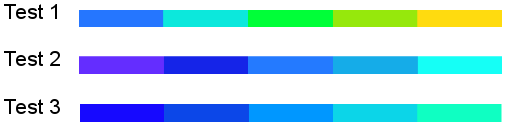
\includegraphics[width=3cm,height=6cm]{spectra.png}
\caption{Spectra}
\label{fig:spectra}
\end{figure}

It is important to understand the dangers of removing test cases. Unless two test cases are exactly the same, it is difficult to guarantee that they are indeed redundant, even if one is a subset of another. Therefore the aim of the project is to identify different approaches that give developers an idea on the number of redundant test cases that are contained within a project. It should allow the developer to run a set of pipelines they specify and view the results on a GUI, allowing manual inspection to determine if they are truly redundant. This means that the tool is useful for gaining an overview and understanding of the condition of the current test suite.

A potential use of the tool is to allow for splitting of any redundant tests into separate test suites allowing for them to be run at different times. For example, one test suite can be run during continuous integration, and the other over night. Ensuring that we are not losing any probability of finding a bug, instead redistributing the test time.

Dr David Pearce is currently writing a language called Whiley, which contains an extended static checking framework in order to eliminate run time exceptions through formal verification techniques. In the compiler module alone, there are roughly 40,000 tests. To reduce this number could result in allowing David Pearce to increase development speed due to a reduction in the time taken to run a large test suite. 
\chapter{Related Work}\label{C:related}

Testing is a critical part to any software engineering process, not only to stop incidents stemming from the the product, but also partially related to the increase in popularity of agile methodologies \cite{chaos}. Many of these methodologies employ test driven development and continuous integration resulting in testing becoming more important throughout the development process. For these reasons there have been research papers that examine the different approaches that can be taken to identify redundant test cases and reduce the size of test suites \cite{wong1995effect, wong1999test, rothermel1998empirical, rothermel2002empirical,koochakzadeh2009test,zhang2011empirical,li2008static}.

It is unclear whether programmatically reducing a test suite's size is worth the tradeoff in the ability to locate bugs.  Wong et al. \cite{wong1995effect, wong1999test} found that test suite reduction does not severely impact fault detection capability. In contrast, Rothermel et al. \cite{rothermel1998empirical, rothermel2002empirical} found that test-suite reduction can severely impact the fault detection capability. This is the reason that our research uses human intuition to have the final say.

A popular technique used in detecting redundancy involves analysing the statement executions, known as coverage information. Maurer, Garousi and Koochakzadeh \cite{koochakzadeh2009test} attempt to answer the question, is coverage based identification enough information to determine redundant test cases? To identify a redundant test case, they state it as being a test case that does not improve a specific criterion. For example, in Figure \ref{fig:venndiagram} we see that according to the coverage data of test cases, T1 ... T5, T4 and T5 are fully redundant as T3 covers the statements that are executed by those tests. This criterion is examining statement coverage. They looked at two other criterion, branch coverage and granularities. Granularity criterion involved splitting the tests into setup, exercise (execution), verify (assert) and lastly teardown then performing analysis over each section. They implemented two different metrics in which both used the criterion described above. These two metrics examined redundancy on at a 1-1 and 1-all relationships. By comparing with manual inspection, they were able to determine the level of false positive and actual redundant tests. Of the redundant tests identified manually, the metrics matched 95\% of those. However, of the tests that were manually identified as being non-redundant, 52\% of these were identified as being redundant by the metrics. They concluded that coverage-based information is vulnerable in giving false-positives when identifying redundant test cases, suggesting common code paths as being the main protagonist. 

\begin{figure}[h]
\begin{center}

\includegraphics[]{VennDiagram.png}
\end{center}
\caption{A Typical Criterion}
\label{fig:venndiagram}
\end{figure}

A technique that Zhang, Marinov, Zhang and Khurshid \cite{zhang2011empirical} examined was the use of a greedy technique in comparison to heuristics with the coverage information. This required a test requirement to be set by the tester, for example using statement coverage. The greedy technique would greedily select a test case that satisfies the maximum number of unsatisfied test requirements and would continue until all the test requirements had been satisfied. So the new test suite will contain exactly the same coverage as the old test suite while removing redundant test cases. This means that if a test subsumed another, then it would always be removed. The heuristic implementation was first conceived by Harrold, Gupta and Soffa \cite{harrold1993methodology} where essential test cases are selected as early as possible. Essential being that only when one test case satisfies a test requirement exclusively. The heuristic approach resulted in the most cost-effective reduction showing that although greedy approach worked, there were better techniques available.

In situations where it is not possible to generate a spectrum to analyse, static analysis can be used to determine the level of redundancy. Robinson, Li and Francis \cite{li2008static} examine the possibility to do this. For the benchmark they use, the test cases are written in a high level automation framework and consist of a list of commands. The commands perform actions such as file copying and loading configurations. To identify redundant test cases they examine the test cases commands as well as the instructions within the procedures that the test case loads. To calculate the similarities between two test cases, they consider three different metrics, Manhattan distance, unigram cosine similarity and bigram cosine similarity. They each were measuring how closely related two tests were based on the sequence of commands and procedures loaded. Their findings were similar to Maurer et al. \cite{koochakzadeh2009test} in that there are a large number of false - positives.

Static checking has several limitations in comparison to dynamic. Firstly, during run-time is when a large part of the paper trail is accessible. Before then the only information available are the method calls. Secondly, it is more difficult to analyse, due to inheritance in many languages adding a complex situation when determining method execution. Static checking therefore would provide useful information in a framework where dynamic data can not be collected and allows for the test cases to be examined in a static fashion such as the one used by Robinson, Li and Francis \cite{li2008static}. Dynamic allows for more data to be collected such as the parameters passed to a method as well as the ability to be executed on more suites. The papers examined looked at the coverage of a test suite at several different criterion levels but none looked at the spectra explicitly. This leaves a potentially useful approach to the problem that may help determine the level of redundancy within a test suite. 
\chapter{Work Done}\label{C:workdone}

\section{Overview}

The ability to trace java unit tests and perform several different analysis metrics has been implemented. For this to be achieved, several factors had to be completed and these are explored in this chapter. The different types of spectra are looked at in Section \ref{S:spectra}. The different types of analysis metrics are explored in Section \ref{S:metrics}. How the tracing is performed is examined in Section \ref{S:trace}, while the creation of the framework is explored in Section \ref{S:framework}. Lastly, how the benchmarks were selected is looked at in Section \ref{S:bench}.

\section{Test Spectra}
\label{S:spectra}

The idea of a spectrum was previously identified in Chapter \ref{C:intro}. A spectrum is some abstraction of the method executions during a test. This allows there to be several different types of spectra. The main three spectra examined are set, list and calling context. An example using the word kitten will be used to show them, where each letter represents a method execution and each letter is from the same parent method.

\begin{itemize}
\item Set of method executions - where every method execution is only taken into account once (Result: 'Kiten')
\item List of method executions - where every method execution is taken into account, including duplicate calls (Result : 'Kitten')
\item Calling Context - for each method call, the data contains a separate node for each call stack that the method was called with \cite{callingcontext} (Result : 'Parent $\rightarrow$ k, Parent $\rightarrow$ i, Parent $\rightarrow$ t ...) 
\end{itemize}
These spectra will be analysed by different metrics to determine the level of redundancy between two tests. This is achieved in Java by examining the stack trace of the method call, where it gives information on the calling tree for that method execution. In the next section, two different analysis metrics are introduced and examined.

\section{Analysis Metrics}
\label{S:metrics}

The first metric is the Levenshtein distance between two tests spectra. This metric is the minimal number of operations that can be done to make one tests spectrum equal to another. These operations are inserting, deleting or substituting method calls and a cost is associated with completing an operation. The max difference is the size of the larger of the two spectra's. The amount of redundancy is calculated by dividing the cost of operations with the max difference in order to normalize the value. This value will be the percentage of tests that are not redundant, we minus this value by 1 to give the redundant level.

If we look at an example using a list spectra, where 'kitchen' is being compared to 'kitten' then we will have to do the following changes.

\todo{Put into a structured table to show more clearly. Unsure how.}
\begin{enumerate}
\item kitten $\rightarrow$ kitcen (Substitution of 't' with 'c')
\item kitcen $\rightarrow$ kitchen (Insertion of 'h' between 'c' and 'e')
\end{enumerate}

This shows the number of operations needed is 2, and the max is 7 as kitchen contains 7 characters. The redundancy is calculated by subtracting 1 from the cost over the max potential cost. So these two words contain 71\% redundant information. 

The second metric was determining the total difference between two spectra. This metric disregarded the calling order of a spectra, which is comparable to looking at the coverage as done in several papers \cite{fraser2007redundancy,koochakzadeh2009test,zhang2011empirical,jeffrey2005test}. The metric sorts the method calls of a spectra in alphabetical order and increments a value by 1 for each difference there is between two tests spectra. Resulting in the total difference between two tests. This value is then divided by the max possible value, which would occur when every method call is different becoming the length of both spectra, to produce a normalized redundancy value. This metric is also minimization.

Using the same spectra example as above, we need to rearrange 'kitchen' and 'kitten' into alphabetical order before calculating the redundancy, 'cehiknt' and 'eikntt' respectively.

\todo{Put into a structured table to show more clearly. Unsure how.}
\begin{enumerate}
\item Remove 'c' from 'cehiknt', increment value by 1
\item 'e' is contained in both, remove from both
\item Remove 'h' from 'hiknt', increment value by 1
\item 'iknt' is contained in both, remove from both
\item Remove 't' from 't', increment value by 1
\end{enumerate}

The total difference between the two is 3. While the max would be if they were both completely different which is 13. The redundancy is calculated by subtracting 1 from the cost over the max potential cost. The outcome being that the two words are 77\% redundant.

Maurer et al. \cite{koochakzadeh2009test} and Robinson et al. \cite{li2008static} found that test cases often had a set of methods that were in every test, such as setup and tear down. These common methods could create false positives. To understand why, a redundant test is one where it is nearly or exactly a replication of another test. Since each method call within an spectra has the same weighting, the more setup and teardown calls made means that the execution stage has decreased weighting overall. So the idea in weighting is to increase the 'importance' of lower frequency method calls by discarding the top 20\% method calls. This weighting will be added into a spectrum, where the spectrum will ignore the top 20\% method calls.

\section{Tracing}
\label{S:trace}

David Pearce's language Whiley is written in Java. Therefore it was decided to use Java to trace a tests spectrum. There are two viable options, the Java Debugging Interface (JDI) or AspectJ. JDI is similar to using an observer pattern. When a method is called, the listening trace class will be notified. In contrast, AspectJ utilises byte code weaving; this is when a piece of code is added to existing code without modifying the code itself. It uses a point cut to identify what code is weaved and where in the code \cite{aspectwiki}. A point cut is made in every method call, this point cut calls a static method in a tracer class, passing it the information about the method execution. AspectJ allows for several methods to achieve tracing through byte code weaving:

\begin{itemize}
\item Compile time:
The classes are compiled with the aspect weaved into them. So that when the jar is executed, the methods have the byte code from the aspect weaved into it already.
\item Load time:
This involves binary weaving deferred until the point in which a class loader will attempt to load in a class file.
\end{itemize}

Load time allowed for ease of use when working with external benchmarks as it only required AspectJ's class loader to be used instead through a command line flag of rebuilding the benchmarks with the AspectJ compiler.

In regard to JDI or AspectJ, AspectJ allows for more ability to choose which methods to record and making it easier to retrieve parameter values, JDI was faster to execute but provided less documentation. The decision to use AspectJ was based off this trade off between more information and performance. The analysis framework was able to be altered to increase the performance of it, so having the extra information that AspectJ gave was more important than an taking less time to execute.

\section{Framework}
\label{S:framework}

The spectrum of every test has to be compared to that of every other test in order to identify redundant test cases. The metrics identified become computationally heavy with thousands of test cases containing a spectrum consisting of tens of thousands of methods calls. To perform an analysis on that scale would take several days. A pipeline combined with time reduction strategies was determined to be the best solution.

A pipeline approach is shown in Figure \ref{fig:pipeline}. The analysing stages can be set by the user within a properties file, where they can select the spectra type, analysis metric to use and level of redundancy for each. This allows execution of reduction strategies before executing more computationally heavy analysis.

\begin{figure}[h]
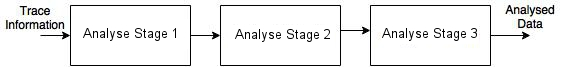
\includegraphics[width=\textwidth]{Pipeline.jpg}
\caption{Trace information goes in at the start of the pipeline. After each stage there will be a reduction of comparisons that the next stage has to complete. The last stages should be the most computationally heavy.}
\label{fig:pipeline}
\end{figure}

There were two approaches that were used to reduce the amount of analysis time. They were - implementing a heuristic and using concurrent execution. 

The heuristic looked at set of method calls, rather than a list. This meant the number of comparisons decreased. Using a 99 percent similarity for the heuristic on the wyc package of Whiley, this decreased the comparisons from stage 1 having 187922 to stage 2 with 232. 

The following illustrates an example of this.

$K,I,T,C,H,E,N \neq K,I,T,E,N,Z $

In this case, the two test cases would not be redundant due to them having a large difference in method calls.

$K,I,T,C,H,E,N \approx K,I,T,C,H,N$

There is a chance that these two may be redundant so it implies more computational heavy analysis should be done, such as analysing the list spectra. 

Concurrent execution was implemented by splitting the test cases up into 8 different parts, each part knew the test cases that it had to compare. A new thread was run to execute the comparisons, making the implementation relatively easy. The concurrent execution lead to a decrease in roughly 2 times the time taken to analyse the spectra's but lead to a trade off in an increased memory usage. This meant concurrent execution was only usable for the smaller bench marks.
Another issue was that for each analysis of a benchmark, the tests had to be rerun, this could take several hours. The solution was to save the spectra data to disk. This ensured that a distributed computing system (ecs grid) could be used to execute data analysis, meaning that 150 analysis jobs could be run at once.

Using reflection will allow for retrieval of parameter values, the use of parameters allows for more certainty about the whether two tests are redundant. The most common use case would involve the use of parameters therefore it was decided to optimize this through storing the data with parameters. The optimization involved saving the parameters with the trace information. If parameters value is set to false, the parameters have to be split off rather than added on. This means that setting the parameters to false would increase the set up time.

\section{Benchmarks}
\label{S:bench}
Suitable benchmarks had to be found to test the different metrics on. They were located by looking at popular java framework's, Github repositories and David Pearce's personal projects. The benchmarks had to meet a criteria where they were Java based, had reasonable number of tests (40+) and were open source. Although there were over ten potential benchmarks, the ability to use them depended on their build process. If they used Maven, it was difficult to create a jar that contained the tests and often meant that the amount of effort needed to get a working benchmark was higher than the benefit from it. This eliminated several potential benchmarks and left the Ant and gradle built projects. In Table \ref{large_test} we see the large bench marks used. These involved bench marks that required more than \todo{TODO} number of comparisons. The type of tests were also taken into consideration.

The current set of benchmarks is as follows:
\begin{table}[]
\centering
\caption{Large Test Suites}
\label{large_test}
\begin{tabular}{|l|l|l|l|}
\hline
{\bf Benchmark}       &  {\bf Number of Tests} & {\bf Type of tests} & {\bf Authors}   \\ \hline
Whiley - Wyc Valid         &       &    End to End      & David J Pearce          \\ \hline
Spring - Core   &       &    Unit Tests      & Community \\ \hline
Metric-x - Core &       &    Unit Tests      & Community \\ \hline
Ant             &       &    Unit Tests      & Community \\ \hline
\end{tabular}
\end{table}

\begin{table}[]
\centering
\caption{Small Test Suites}
\label{small_test}
\begin{tabular}{|l|l|l|l|}
\hline
{\bf Benchmark}   & {\bf Number of Tests} & {\bf Type of tests} & {\bf Authors}  \\ \hline
Jasm              &             &    End to End      & David J Pearce \\ \hline
Imcache &           &    End to End        & Community \\ \hline
\end{tabular}
\end{table}

\chapter{Results and Discussion}\label{C:results}\label{C:evaluation}

The following section reports on the outcome of several experiments that explore the use of our framework through a realistic benchmark suite. The key factors of interest are -- the time taken, number of comparisons, the types of redundant tests identified and the overall cost of performance (time) vs precision (tests identified \& types identified). \todo{Link back to req?}

There are two points that the reader needs to be aware of. Firstly, in the significant tables below, a `+' represents that significant increase, `-' significant decrease and `=' represents no significant difference. Secondly, the graphs are displayed using a logarithm scale.

\section{Method}

The experiment method is key to producing believable and reproducible results. Before the experiment could be conducted, the data for each benchmark had to be retrieved. This involved setting the benchmark up locally and then executing the tests with the AspectJ class loader. The data was then run on a grid computing system. After the results had been returned, a Wilcoxon signed rank test \cite{wilcoxon1945individual} was used to determine whether the results were significantly different or not. The significant level used was 95\% with a null hypothesis of the two samples median being equal. Overall, a total of seven different property settings were run per benchmark with each property setting being run 30 times.

The goals of this paper as mentioned in Section \ref{C:intro} are the creation of a framework to identify redundant test cases and experimenting the different techniques on realistic benchmarks. The rest of this section explores the experiments conducted to give guidance to the users of the framework.

\section{Environmental Methodologies}
\label{enviro}
As previously discussed in Section \ref{performanceEvalBG} there are a variety of challenges that present themselves when using Java to evaluate performance. These challenges are discussed throughout the following section.

\subsection{Grid Computing}
A grid computing system was used to execute the data analysis, with a total of 150 jobs queued on the grid at a single time. When using a grid system it is important to ensure that all the machines used are the same for every experiment. The grid allowed for particular types of machines to be specified -- 8gb total ram, Linux 4.0.5 64 bit system and an i5.

\subsection{Measuring Time}
The time taken is an important variable in evaluating the performance of a tool. In Java, this can be achieved by accessing a system method that returns the total time in milliseconds from 1970 00:00:00 UTC to the current time. Taking this time before the analysis, and subtracting from the time after the analysis gives the total time taken. This notation of time is defined as wall clock time. Utilising a grid system presents difficulties with using the wall clock time to measure the time taken. 

As mentioned in Section \ref{C:related}, when a job is run on the grid system, there is potential for the machine to be paused. If wall time were to be used, the time that the process is paused would also be included. To resolve this issue, the notation of CPU time was used. The CPU time is the measure of time in nanoseconds that the computer program spent on the CPU. Another issue in regard to time taken if a user logs in during analysis, is the programs RAM could potentially be moved into virtual memory. This is dependent on the amount of RAM that the user needs. Both these issues were limited by running the tests overnight when users were unlikely to log.

When measuring the time taken to analyse, the start up cost was not taken into account. Running up to 150 jobs meant that a large number of applications would be attempting to access a single data file at a single time. This stress on the system introduces a large amount of non-deterministic behaviour. Removing the start up cost avoided this issue.

\subsubsection{Heap Size}
The heap is the location that the JVM uses to store objects that are produced during the execution of an application. The amount of heap that was allocated to the JVM was 6gb for every benchmark over every run.

\subsection{Software Environment}

A concurrent-mark-sweep garbage collection strategy (default) was used. This approach uses multiple threads to scan the heap, mark unused objects and recycle them \cite{oracle2015}. It allows for a high throughput however, tends to use more CPU time than other strategies. This was deemed worth the trade off as memory was the bottleneck rather than CPU and increasing the throughput was more important.

\section{Benchmarks}
\label{S:bench}
The benchmarks had to be realistic real world projects. They were located by looking at popular Java frameworks, Github repositories and David Pearce's personal projects. For a benchmark to be considered, it had to be Java based, have a reasonable number of tests (40+) and was open source, while Ant and Gradle built projects were favoured due to their easier build process.

A variety of test types and sizes of benchmarks were examined. A range of sizes were used in order to fully evaluate the framework. The two ranges of benchmark sizes can be found in Table \ref{large_test} and Table \ref{small_test}, large and small respectively. Although method execution details approach is aimed toward larger test suites, it would be expected that size will have no correlation to the metrics examined. A range of test types were also chosen, David J Pearce's projects contain end to end tests which run through a whole module at once, while the rest attempt to test units of code at a time. Having a range of test types gives a wider evaluation view and gives insight into potential situations where different settings may not be helpful in achieving the aim.

The larger benchmarks that produced up to 100,000 method calls per test required a large amount of memory to store the details during data retrieval. Without the use of a database, this limited the number of test cases that could be collected. Whiley and Ant were the benchmarks that did not have all there tests executed.  

\begin{table}[]
\centering

\begin{tabular}{|l|l|l|l|}
\hline
{\bf Benchmark}       &  {\bf Number of Tests} & {\bf Type of tests} & {\bf Authors}   \\ \hline
Whiley - Wyc         &       &    End to End      & David J Pearce          \\ \hline
Spring - Core   &       &    Unit Tests      & Community \\ \hline
Metric-x - Core &       &    Unit Tests      & Community \\ \hline
Jasm              &             &    End to End      & David J Pearce \\ \hline

\end{tabular}
\caption{Large Test Suites}
\label{large_test}
\end{table}

\begin{table}[]
\centering
\begin{tabular}{|l|l|l|l|}
\hline
{\bf Benchmark}   & {\bf Number of Tests} & {\bf Type of tests} & {\bf Authors}  \\ \hline
Ant             &       &    Unit Tests      & Community \\ \hline
Imcache &           &    End to End        & Community \\ \hline
\end{tabular}
\label{small_test}
\caption{Small Test Suites}
\end{table}

\section{Experiment \rom{1} - Pipeline Length Comparison}
\label{sec:pipelineEva}

\subsection{Motivation}
The pipeline size has impact on each factor of interest. Selecting a pipeline too small or too large will have varying negative effects on these. This experiment explores this trade off and the number of pipelines that should be used with the benchmarks.

\begin{hyp}
Increasing the number of pipeline's improves the factors of interest
\end{hyp}

\begin{hyp}
Increasing the number of pipeline's leads to no difference between the output redundant test cases
\end{hyp}

\subsection{Settings}
There were two different pipeline size's tested, two and three respectively. For both size's, the final pipeline stage was the same. It is noted that a single pipeline comparison was left out due to the amount of memory and time taken to finish analysing.

\begin{itemize}
\item Difference between runs: Pipeline size
\end{itemize}

\subsection{Results}

The significant table for comparing the use of pipeline of size two vs size three is shown in Table \ref{pipelinesig}. It shows that there was a mixture of results for the total time taken to analyse the data. Metrics-x, Ant, Spring and Jasm performed significantly better with a pipeline of size three in comparison to size two. Imcache had no significant difference and Whiley performed significantly worse with a pipeline of size three in comparison to size two. Every benchmark has no significant difference between the number of redundant tests identified, every benchmark produced the exact same number of redundant tests in both pipeline size of two and three.

A chart showing how each benchmark reacted to the change in the pipeline size is shown in Figure \ref{fig:pipelinegraph}. It shows the number of test case comparisons that the final stage of the pipeline has to conduct.

\begin{table}[h]
\centering
\begin{tabular}{|l|l|l|}
\hline
{\bf }          & {\bf Total Time} & {\bf Redundant Tests Identified} \\ \hline
{\bf Whiley}    & +                & =                           \\ \hline
{\bf Jasm}      & -                & =                           \\ \hline
{\bf Ant}       & -                & =                           \\ \hline
{\bf Spring}    & -                & =                           \\ \hline
{\bf Imcache}   & =                & =                           \\ \hline
{\bf Metrics-x} & -                & =                           \\ \hline
\end{tabular}
\caption{A table showing the significant relationship between the use of pipeline of size two with pipeline of size three for each benchmark}
\label{pipelinesig}
\end{table}

\begin{figure}[h]
\begin{center}
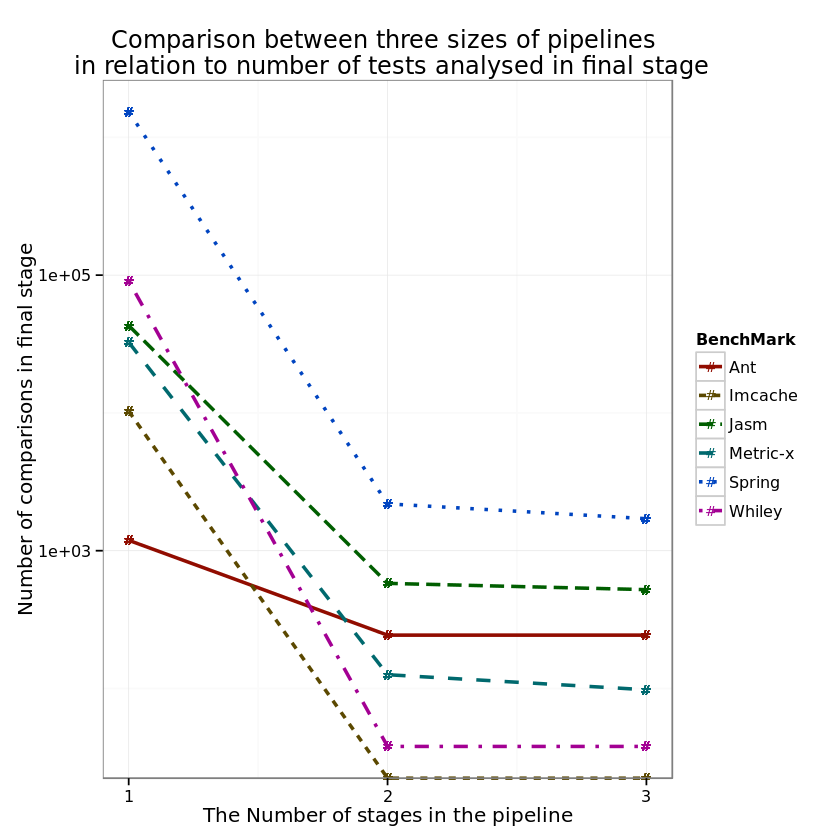
\includegraphics[height=10cm, width = 14.5cm]{Pipeline.png}
\end{center}
\caption{A figure showing the effect that using pipelines has on the number of comparisons that the final stage (Most computationally heavy) has to do.}
\label{fig:pipelinegraph}
\end{figure}

\subsection{Discussion}

The first hypothesis states an increase in the pipeline size will improve the factors of interest. An increase in the pipeline size aimed to reduce the number of comparisons that the next stage had to perform. This in turn decreased memory and time taken. Immediately it becomes clear that that pipeline size does improve the factors, but doesn't scale in every benchmark. This becomes visible when examining Figure \ref{fig:pipelinegraph}. Every two or three stage pipeline is a significant improvement on a single stage, however the majority of benchmark's perform better for a two stage over a three. These results imply that the benchmarks that took less time using a two stage, were spending more time on the second stage than they were saving from the reduced number of comparisons in the third stage. 

Two situations which would cause more time to be spent on the second stage than was saved in the third stage are proposed. Firstly, each benchmark had it's own level of redundancy that was being looked for, this was dependent on how each benchmark reacted to different levels. Benchmarks with unit tests needed to have a higher level in comparison to benchmarks with end to end. Since each benchmark had their own percentage, this implies that each benchmark also has its optimal settings for the second pipeline. The settings were chosen by experimenting with different options, therefore a inefficient second pipeline would have contributed to it.

The second reason is that there may be little difference between the second pipeline and third pipeline. An example is shown in Appendix \ref{fig:pipelinecomp}. Examining the three stage pipeline, it shows the first pipeline causes a large reduction in the number of comparisons needed implying that the tests are highly separable. Inserting the second stage, a limited amount of reduction occurs while being computationally heavy and passes the majority of test cases into the third and most computationally heavy stage. \todo{Talk about cost here.} This leads to a situation where the number of identified redundant test cases has little change from stage two to three. This leads me to accept the first hypothesis, that increasing the pipeline size improves the factors of interest, however the optimal length is different for each benchmark.

The second hypothesis is that there is no difference between the number of output test cases. As expected, each benchmark had no significant change. If there were a change between the two pipelines with the same final stage settings could imply two things. Firstly, there is a bug in the code. Secondly, the second pipeline stage is more specific than the last. Since both the second stage and third stage share the same final stage, this would cause the last stage to be redundant and the redundant tests different to that of the two stage pipeline. 

\section{Experiment \rom{2} - K Depth Comparison}
\label{kdepthcomp}
\subsection{Motivation}
One of the abilities of the framework is to trace the K depth specified. This experiment is to determine the impact that altering the depth of K has on the overall cost. 

\begin{hyp}
Increasing the K Depth improves the precision is worth the trade off in performance decrease.
\end{hyp}

\subsection{Settings}
There are three K depth's explored, one, two and three respectively.

\begin{itemize}
\item Difference between runs: K Depth
\end{itemize}

\subsection{Results}
Ant, Whiley and Spring appear to be the most responsive to the depth of K as shown in Figure \ref{fig:kdepthgraph} while the rest have limited change. Appendix \ref{fig:kdepthtime} shows the differences in time taken. Overall, for every benchmark there wasn't a large amount of change between them however it shows that as the K depth increases, the time taken increases.

\begin{figure}[h]
\begin{center}
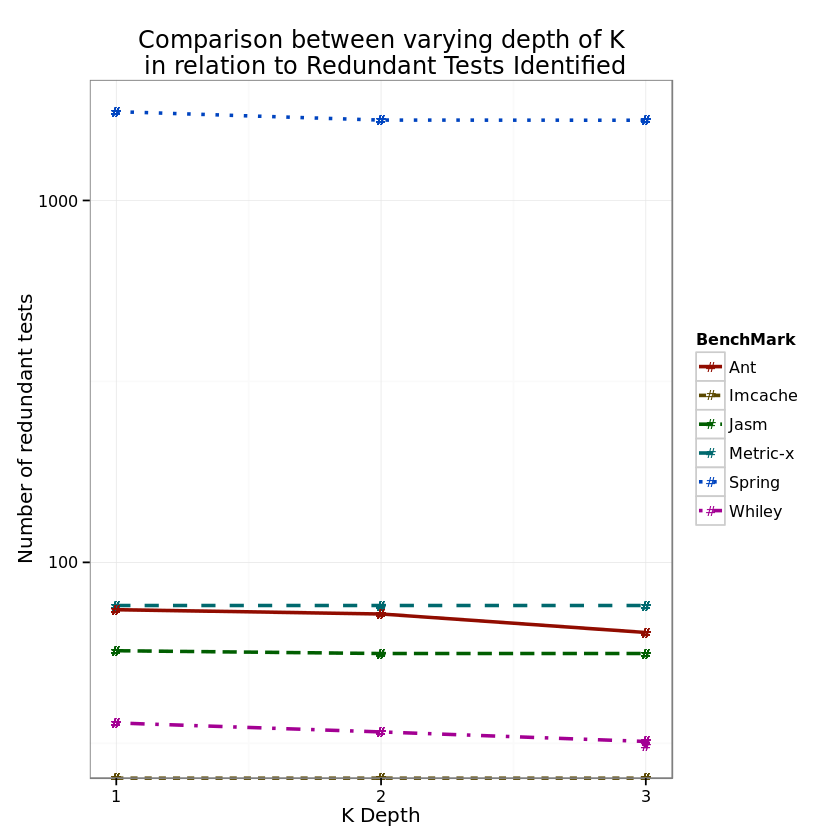
\includegraphics[height=10cm, width = 14.5cm]{KDepth.png}
\end{center}
\caption{A figure showing the effect that a change in the depth of the calling context has on the number of redundant tests are identified.}
\label{fig:kdepthgraph}
\end{figure}

\subsection{Discussion}
Increasing the depth of the calling context increases the amount of data that is analysed, intuitively making it more difficult for test cases to be the same. This should be reflected through a reduction in the overall tests identified. The extra data used is going cause extra analysis, this implies an increase in the time taken as calling context depth increases. It is expected that the precision increase is worth the performance decrease.

Examining Figure \ref{fig:kdepthgraph}, it shows that the number of redundant tests is only slightly decreased as the K depth increases. This may show several things. Firstly, it may imply that when no other settings such as weighting or parameters are used, then the depth has limited effect on the redundant test cases identified. Secondly, the number of comparisons that were output from the first pipeline stage may cause there to be a limited differentiation. When the first pipeline stage outputs a low number of comparisons, then the final number of redundant tests identified would be similar regardless of the K depth specified, similar to the situation in Section \ref{sec:pipelineEva}. This occurs in Whiley and Metric-x. 

Increasing the depth of K has varying effect's on the time taken to analyse a benchmark. The differences are shown in Appendix \ref{fig:kdepthtime}. It shows that Ant, Imcache and Whiley have larger differences than the rest, however in the perspective of time these equate to around half a minute difference. Although increasing the depth has an smaller effect than expected on precision, the impact on time taken isn't substantial. Taking this into account, I can accept the hypothesis with the results implying that for some projects the calling context does not have to be particularly deep.

\section{Experiment \rom{3} - Parameter Comparison}
\label{sec:param}

\subsection{Motivation}
Parameters show the different contexts that a method was being called in. Retrieving this information gives us more confidence in determining whether two tests are redundant. This shows the importance of parameters and the experiment explores the increase in performance and precision.

\begin{hyp}
Utilising parameters increase the time taken of the framework in comparison to a standard three stage pipeline
\end{hyp}

\begin{hyp}
Utilising parameters increase the precision of the framework in comparison to a standard three stage pipeline
\end{hyp}

\subsection{Settings}
The use of parameters is compared directly to the pipeline size three settings.

\begin{itemize}
\item Difference between runs: Parameters used during analysis
\end{itemize}

\subsection{Results}
The significant table for comparing parameters and no parameters is shown in Table \ref{parametersig}. It shows that there was a negative relation (increase) for every benchmark in regard to time taken. Every benchmark had a significantly positive effect (decrease) on the number of redundant test cases identified. This is not the case in Imcache due to it having zero redundant test cases identified in both, therefore no difference between the two.

\begin{table}[h]
\centering
\begin{tabular}{|l|l|l|}
\hline
{\bf }          & {\bf Total Time} & {\bf Redundant Tests Identified} \\ \hline
{\bf Whiley}    & +                & -                           \\ \hline
{\bf Jasm}      & +               & -                          \\ \hline
{\bf Ant}       & +                & -                           \\ \hline
{\bf Spring}    & +                & -                           \\ \hline
{\bf Imcache}   & +                & =                           \\ \hline
{\bf Metrics-x} & +                & -                           \\ \hline
\end{tabular}
\caption{A table showing the significant relationship between the use of parameters and no parameters for each benchmark}
\label{parametersig}
\end{table}

\begin{figure}[H]
\begin{center}
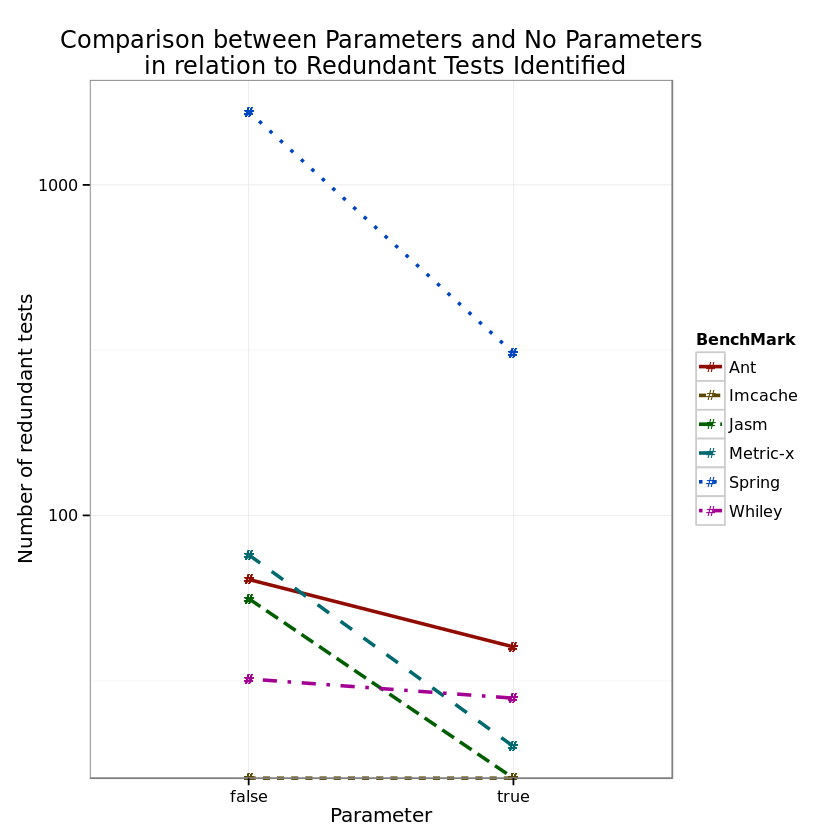
\includegraphics[height=10cm, width = 14.5cm]{Parameters.png}
\end{center}
\caption{A figure showing the effect that using parameters has on the number of redundant tests are identified.}
\label{fig:paramgraph}
\end{figure}

\subsection{Discussion}
Two factors have to be taken into account when discussing the impact of parameters on the time taken. Firstly, it is intuitive that analysing the extra data generated increases the time. The amount of increase is interesting, parameters only add extra computation when the method execution of the given K is exactly the same. For example, if test execution is $A ->  B ->  C$ is compared to $A ->  B ->  F$. Then the parameter won't be taken into account and therefore have limited effect on the time taken. 

The amount of time that the VM spends garbage collecting would also increase the time taken, due to increased amount of information in memory, the garbage collection process will have to execute more frequently for the analysis to continue to run. This would cause non-deterministic attributes to be increased. Examining Appendix \ref{fig:paramtime} -- Ant, Imcache, Jasm and Spring appear to affected by this due to the increased variance. This creates the hypothesises that parameters decrease the precision and increase the total time taken. 

The significant Table \ref{fig:paramgraph} matches what is expected. For every benchmark, using parameters significantly increases the time taken. Examining Appendix \ref{fig:paramtime} shows how the benchmarks react with more detail. The most interesting would be JASM. Without parameters, it analyses the data in less than one minute, with parameters, it takes just under five minutes. This may be indicative of the results discussed in Section \ref{kdepthcomp}. With K depth having little effect on a reduction in comparisons, the number of tests that match the K depth of three is higher than expected. This effect led to parameter information being examined more often, sequentially causing an increase in time taken. \todo{A factor that may have an accumulate effect} is related to the setup methods. If the set up methods are a large majority of the method calls, and match each other for the K depth, this would further increase the time taken. This allows us to accept hypothesis 4.

Every benchmark caused a significant decrease in the number of redundant test cases. Looking at Figure \ref{fig:paramgraph} shows that every benchmark reacted with a substantial decrease in redundant tests identified, with Whiley being the least affected. This reiterates the discussion in Section \ref{kdepthcomp} that K depth is not enough of a factor to identify redundant test cases. It is expected that identified tests decreases, inspecting Table \ref{whileycoding} and \ref{metriccoding} gives insight into the types of tests identified. The Whiley benchmark coding shows that parameters remove the limited redundant tests as well as different array values. The Metric-x coding shows the influence that parameters has. Parameters reduce the number of the different parameter value tests identified substantially, from 52 to 8. These coding allow us to accept hypothesis 3.

\section{Experiment \rom{4} - Weighting Comparison}
\label{sec:weight}

\subsection{Motivation}
Utilising weighting is an attempt to remove any false positive tests identified. The experiment attempts to identify if weighting has any potential to remove these false positives, while exploring the impact on performance.

\begin{hyp}
Weighting decreases the number of false positives compared to a standard three stage pipeline
\end{hyp}

\begin{hyp}
Weighting decreases the time taken compared to a standard three stage pipeline
\end{hyp}

\subsection{Settings}
The use of weighting is compared directly to the pipeline size three settings.

\begin{itemize}
\item Difference between runs: Weighting Used
\end{itemize}

\subsection{Results}
The significant table for comparing the use of weighting is shown in Table \ref{weightingsig}. There are a mixture of results in regard to the total time taken -- Whiley, Ant and Imcache had a significantly negative relation and weighting increased the time taken to analyse. Jasm, Spring and Metric-x had a significantly positive relation and weighting decreased the time taken to analyse. The majority -- Whiley, Ant, Jasm and Metrics-x had a significantly positive relation in regard to the number of redundant tests identified, showing a decrease in the number identified when weighting was applied. Spring was the only benchmark where weighting had a significantly negative impact.

\begin{table}[h]
\centering


\begin{tabular}{|l|l|l|}
\hline
{\bf }          & {\bf Total Time} & {\bf Redundant Tests Identified} \\ \hline
{\bf Whiley}    & +                & -                           \\ \hline
{\bf Jasm}      & -                & -                           \\ \hline
{\bf Ant}       & +                & -                           \\ \hline
{\bf Spring}    & -                & +                           \\ \hline
{\bf Imcache}   & +                & =                           \\ \hline
{\bf Metrics-x} & -                & -                           \\ \hline
\end{tabular}
\caption{A table showing the significant relationship between the use of weighting and no weighting for each benchmark}
\label{weightingsig}
\end{table}


\begin{figure}[h]
\begin{center}
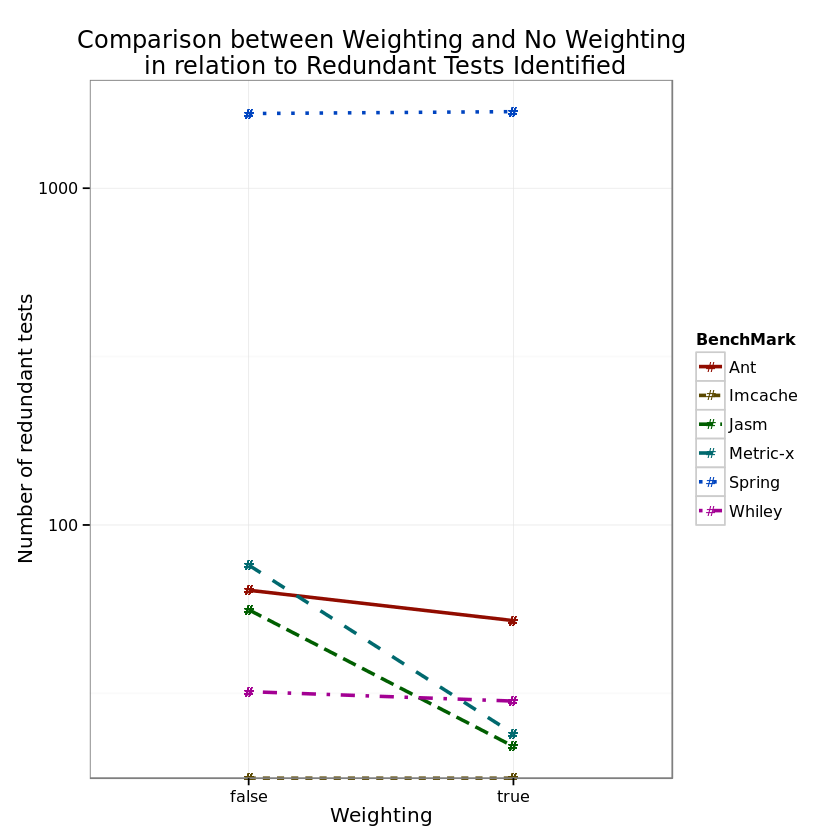
\includegraphics[height=10cm, width = 14.5cm]{Weighting.png}
\end{center}
\caption{A figure showing the effect that using weighting has on the number of redundant tests are identified.}
\label{fig:weightgraph}
\end{figure}

\subsection{Discussion}
As previously discussed in Section \ref{C:related}, much of the related work encountered difficulties with test cases sharing setup and teardown method calls, resulting in a high false positive rate. Intuitively this makes sense when the test cases are small in comparison to the setup and teardown methods where the setup and teardown methods are a larger majority of the tests data. The approach of removing a portion of the most executed method calls meant that the amount of data that would be compared decreases. This should reflect onto the results by showing a decrease in the time taken, as per hypothesis 7. The effect that it has on the number of redundant test cases should be dependent on the benchmark when weighting is used. This is because removing the most common tests should imply an decreased false-positive rate, but also may increase the number of actual redundant tests picked up. To examine the cause effect of weighting, the precision to validate or invalidate hypothesis 6.

Table \ref{weightingsig} shows a mixture of results in regard to the total time taken. Two out of the three benchmarks that had a significant increase in the total time were small benchmarks. This may imply that the size of the benchmark has some relation to the effect of weighting on the time taken. One reason may be that weighting is calculated once per test case per analysis stage. The weighting calculation has a linear relation with the number of test cases. In comparison, every test case is compared to every other, therefore a factorial relation with the number of test cases. Since the factorial relation is closer to linear, the smaller the number of redundant test cases. Then the smaller the number, the more impact the linear weight calculation has on the overall time taken. This may explain a relation between size and time taken. Examining the overall impact from weighting on the time taken in Appendix \ref{fig:weighttime} allows us to invalidate hypothesis 7 as there is no general consensus between benchmarks.

A reduction in the false positive rate was weightings primary goal. Spring was the only benchmark that significantly increased the number of redundant test cases identified. The other benchmarks had a significant decrease. At first, this makes it appear that by using weighting it may solve some of the issues that were identified in \cite{koochakzadeh2009test} \cite{li2008static}. To confirm this, examining Table \ref{whileycoding} and \ref{metriccoding} will give insight into the effect of weighting. Comparing the two columns for the Whiley coding, Pipeline 2 and Weighting, the only difference is the removal of the two limited redundancy test cases that were picked up by Pipeline 2. The weighting is able to remove the test cases that have similar set up and tear down methods, but fails to reduce the number of other redundancies. By removing the method executions that were common throughout the benchmarks, this lead to a decrease in false-positive tests identified. The Metric-x coding paints a similar story. Weighting reduces the number of parameter value redundancies identified as well as the limited redundancies however does not completely remove them. This is interesting and implies that the number of setup and tear down methods that remained in the data analysed was still a large portion of the data. We are able to accept hypothesis 6, although work remains to improve the weighting method to remove redundant tests completely.


\section{Experiment \rom{5} - Weighting and Parameter Comparison}

\subsection{Motivation}
Combining weighting and parameters is an attempt to reduce the number of false positives, and at the same time increasing the confidence of the redundant tests being redundant. 

\begin{hyp}
A combination of weighting and parameters increases the precision in comparison to weighting and parameters separately
\end{hyp}

\subsection{Settings}
The use of weighting with parameters is compared directly to the pipeline size three settings.

\begin{itemize}
\item Difference between runs: Weighting and Parameters
\end{itemize}

\subsection{Results}
The relevant significance table is shown in Table \ref{weightingparamsig} showing a comparison between the combination and pipeline of size two. It shows that for every Benchmark apart from Imcache, there was a negative relation for the time taken, showing that the time increased when using weighting and parameters for the majority of benchmarks. In contrast to this, every benchmark had a positive relation to the number of redundant tests identified. Figure \ref{fig:weightingparamgraph} indicates the number of tests identified for each benchmark in comparison to weighting and parameters separately. Each benchmark reacted differently to the use of weighting and parameters combined -- Spring, Jasm and Metric-x had large decreases compared to the weighting with the rest being similar between the three types. 

\begin{table}[h]
\centering

\begin{tabular}{|l|l|l|}
\hline
{\bf }          & {\bf Total Time} & {\bf Redundant Tests Identified} \\ \hline
{\bf Whiley}    & +                & -                           \\ \hline
{\bf Jasm}      & +                & -                           \\ \hline
{\bf Ant}       & +                & -                           \\ \hline
{\bf Spring}    & +                & -                           \\ \hline
{\bf Imcache}   & -                & =                           \\ \hline
{\bf Metrics-x} & +                & -                           \\ \hline
\end{tabular}
\caption{A table showing the significant relationship between the use of weighting with parameters and pipeline size two for each benchmark}
\label{weightingparamsig}
\end{table}

\begin{figure}[h]
\begin{center}
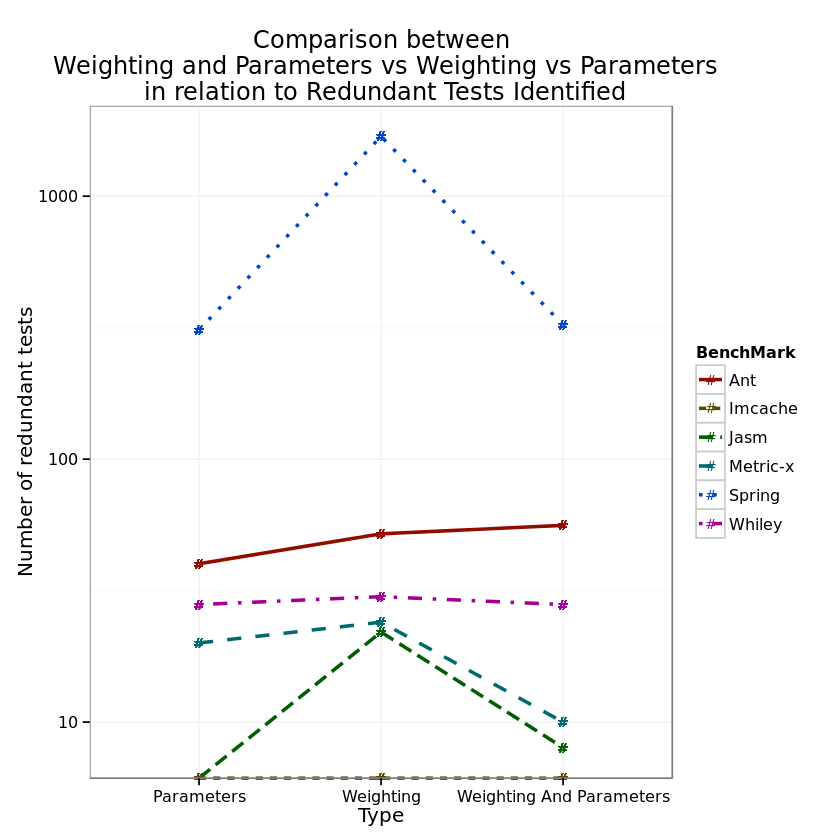
\includegraphics[height=10cm, width = 14.5cm]{WeightNParamVAll.png}
\end{center}
\caption{A figure showing the effect that using weighting and parameters has on the number of redundant tests are identified.}
\label{fig:weightingparamgraph}
\end{figure}

\subsection{Discussion}
Using parameters to increase the confidence and weighting to remove common method executions should increase the precision of the framework. To appraise the combination, Figure \ref{fig:weightingparamgraph} displays the comparison between each of the three types. Weighting identified more redundant tests in every benchmark but Ant. Parameters produce similar results to the combination, apart from in Jasm and Metric-x. Whiley coding in Table \ref{whileycoding} show no difference between parameters and the combination.Metric-x's coding Table \ref{metriccoding} hints that the combination may have some appeal by removing all eight limited redundancy tests. At the same time, the similar tests are also removed which is a negative outcome. This suggests that the combination improves the precision for some benchmarks, but not for others. This conclusion means hypothesis 8 can not be accepted. 

Combining weighting and parameters presents interesting time taken results. Table \ref{weightingparamsig} shows that it is nearly identical to the parameters significance table with the only exception being that the Imcache benchmark changed from significant increase in time to a significant decrease in time. This indicates that parameters have a stronger effect than weighting on the final outcome. This is an unexpected result. As previously discussed in Section \ref{sec:param}, one of the reasons that parameters increase the time taken is due to the similar setup and tear down method calls. With weighting removing a large portion of the common method executions it would be expected to cause a decrease in the number of comparisons using parameters. Looking at Appendix \ref{fig:weightparamvparamtime}, this appears to be true for Jasm, Metric-x, Spring and Imcache. However, for Whiley and Ant benchmarks the time to calculate the weighting information is taking longer than the comparisons saved. 

\section{Redundant Test Case Coding}

\begin{table}[h]
\centering

\begin{tabular}{|l|l|l|l|l|}
\hline
                          & \multicolumn{4}{c|}{{\bf Whiley}}                                                             \\ \hline
{\bf Types of redundancy} & \multicolumn{1}{c|}{{\bf Pipeline 2}} & {\bf Weighting} & {\bf Parameters} & {\bf Parameters and Weighting} \\ \hline
Different Equation Value  & 6                                     & 6               & 6                & 6                \\ \hline
Different Equation Sign   & 8                                     & 8               & 8                & 8                \\ \hline
Different Array Values    & 2                                     & 2               & 0                & 0                \\ \hline
Same                      & 10                                    & 10              & 10               & 10               \\ \hline
Limited Redundancy        & 2                                     & 0               & 0                & 0                \\ \hline
Rearranged Equation       & 2                                     & 2               & 2                & 2                \\ \hline
Extra if statement        & 2                                     & 2               & 2                & 2                \\ \hline
                          &                                       &                 &                  &                  \\ \hline
{\bf Total}               & 32                                    & 30              & 28               & 28               \\ \hline
\end{tabular}
\caption{A table displaying a list of coding's for the Whiley Benchmark for four of the different techniques used.}
\label{whileycoding}
\end{table}


\begin{table}[]
\centering
\begin{tabular}{|l|l|l|l|l|}
\hline
                             & \multicolumn{4}{c|}{\textbf{Metric-X}}                                                              \\ \hline
\textbf{Types of redundancy} & \textbf{Pipeline 2} & \textbf{Weighting} & \textbf{Parameters} & \textbf{Parameters  And Weighting} \\ \hline
Different Parameter Value    & 52                  & 10                 & 8                   & 4                                  \\ \hline
Different Object Type        & 6                   & 2                  & 2                   & 0                                  \\ \hline
Different Array Values       & 8                   & 6                  & 4                   & 6                                  \\ \hline
Similar                      & 2                   & 2                  & 0                   & 0                                  \\ \hline
Limited Redundancy           & 8                   & 4                  & 6                   & 0                                  \\ \hline
\textbf{}                    &                     &                    &                     &                                    \\ \hline
\textbf{Total}               & 76                  & 24                 & 20                  & 10                                 \\ \hline
\end{tabular}
\caption{A table displaying a list of coding's for the Whiley Benchmark for four of the different techniques used.}
\label{metriccoding}
\end{table}

\chapter{Evaluation}\label{C:evaluation}

\section{Pipeline Length Comparison}

An interesting result was the impact of the length of the pipeline had on the total time taken to analyse the data. The idea of the pipeline was to decrease the amount of comparisons that the each stage in the pipeline has to do. This in turn meant less memory consumption and time taken for the more computationally heavy stages. Looking at the results show that in most cases, having two pipeline stages meant a significantly decreased total time taken to analyse over a pipeline with three stages. Intuitively, this may go against what would make sense. Looking at Figure \ref{fig:pipelinegraph}, it shows that there is a major decrease in the number of comparisons that the last stage does between one stage and two or three stages. However, between two and three stages there is limited differences. These results imply that the test cases that took less time using a two stage, were spending more time on the second stage than they were saving from the reduced number of comparisons during the third stage. 

There would be two different reasons that this result may occur. Firstly, as discussed in \todo{DISCUSS IN AN ABOVE CHAPTER.}, each benchmark had it's own level of redundancy that was being looked for, this was dependent on the size of the test cases of each. As benchmarks with smaller test cases needed to have a higher level of redundancy in comparison to benchmarks with larger test cases, as this meant they would have roughly the same percentage of difference. Since each benchmark had their own percentage, this implies that each benchmark also has their optimal settings for the second pipeline. The settings were chosen by experimenting with different options. Therefore, not using a near optimal second pipeline could have contributed to it. \todo{Need to explain it better}

The second reason is that there may be little difference between the second pipeline and third pipeline. For example, if the first pipeline reduces the number of comparisons needed to 50, then there is a limited number of comparisons that a second pipeline can remove. This leads to a situation where the number of identified redundant test cases is similar for both pipelines.

As expected of the redundant tests identified, for each benchmark there was no significant change. If there were a change between the two pipelines with the same final stage settings could imply two things. Firstly, there is a bug in the code. Secondly, for the three stage pipeline, the second stage is being more specific than the last. This would cause the last stage to be redundant and the redundant tests different to that of the two stage pipeline.

\section{K Length Comparison}

Increasing the depth of the calling context means adding more data to the test information used to do the analysis, intuitively making it more difficult for test cases to be the same. This should mean there is a decrease in the number of comparisons as the calling context depth increases. It also means that more data is going to have to be looked at which implies an increase in time as calling context depth increases.

Examining Figure \ref{fig:kdepthgraph}, it shows that the number of redundant tests is only slightly decreased as the K depth increases. This may show several things. Firstly, using a depth of 1 is enough to separate the majority of test cases from each other and shows the redundant test cases with some false positives. This is not likely to be the answer. The reason being that this would make sense for some of the bench marks, however for it to occur to every benchmark makes it appear to be another reason. This other reason is likely to be due to the settings deployed in this comparison. Neither parameters or weighting was selected in the settings, as will be discussed in Sections \ref{sec:param} and \ref{sec:weight} these two setting have a large impact on the number of redundant tests. Another issue could be revolving around the number of comparisons that were output from the first pipeline stage. If the first pipeline stage output a low number of comparisons, then the comparisons output would more likely to be similar regardless of the K depth specified.

\todo{Maybe look at a coding for the different types of tests identified. What types does lower K mean more likely to pick up ?}
\todo{Discuss what the time taken. Get the data again using the specified K Value. Talk to roma about what type of graph to show the time taken}
\todo{Calculate the significant differences ? }

This implies that for some projects the calling context does not have to be particularly deep.



\section{Parameter Comparison}
\label{sec:param}
Intuitively, taking into account for parameters of method calls would increase the time taken to calculate the level of redundancy due to the extra amount of data. However, parameters only add extra computation when the method execution of the given k is exactly the same. \todo{Should I describe this more?} A larger calling context would mean that it would be more difficult for two tests to match. Matching with a K value of three would be expected to be a rare occurrence in the scale of a benchmark. The parameters can be large and hold a lot of information therefore if the K value matches, then matching parameters may incur a large cost. Taking into account this extra information, it would make sense that the number of redundant tests identified would decrease, but the total time taken would increase. 

Looking at the significant Table \ref{fig:paramgraph}, this matches what is expected to occur. For every benchmark, using parameters significantly increases the time taken. This may imply that the number of tests that match the K value of three was higher than expected, causing more computations to look at the parameter information.

Every benchmark caused a significant decrease in the number of redundant test cases. This backs up the implication that there were more situations where a K depth of three matched than expected meaning that parameters had a significant effect on the redundant tests identified. 

\todo{Test on Calling context = 2 ? Look at significant differences}

\section{Weighting Comparison}
\label{sec:weight}
As previously discussed in \todo{section 2 and 3} many of the other papers encountered difficulties when test cases shared setup and teardown method calls, meaning that some of the methods picked up caused a high false - positive rate. Intuitively this makes sense when the test cases are small or the setup and teardown is large, meaning the setup and teardown methods make up a larger majority of the test calls. By taking the approach of removing a portion of the most executed method calls meant that the amount of data that would be compared decreases. This should reflect onto the results by showing a decrease in the time taken. The effect that it has on the number of redundant test cases should be dependent on the benchmark when weighting is used. This is because removing the most common tests should imply an decreased false-positive rate, but also may increase the number of actual redundant tests picked up. Therefore, depending on which on the two variables outweighs the other, will result in an increase or decrease in the number of redundant test cases identified.

Looking at the results in Table \ref{weightingsig}, it shows there was a mixture of results in regard to the total time taken. Two out of the three benchmarks that significantly increased in total time were from the small benchmarks. This may imply that the size of the benchmark is related to the effect of that weighting has on the time taken. The reason is, weighting is calculated once for each test case at the start of the pipeline stage. This weighting calculation can take a varying length of time, depending on the number of test cases. Since the weighting is linear in relation to the number of test cases, however, the comparisons is factorial in relation to the test cases. This shows that calculating the weighting for smaller benchmarks may take more time than it saves. However, the goal of weighting is not to save time, but it is to reduce the number of false positives.

Spring was the only benchmark that significantly increased the number of redundant test cases identified. The other benchmarks had a significant decrease. At first, this makes it appear that by using weighting it may solve some of the issues that were identified in \cite{koochakzadeh2009test} \cite{li2008static}. To confirm this, examining Table \ref{whileycoding} will give insight into the effect of weighting. Comparing the two columns, Pipeline 2 and Weighting it shows the only difference is a removal of the two limited redundancy test cases that were picked up by Pipeline 2. The weighting is able to remove the test cases that have similar set up and tear down methods, but fails to reduce the number of other redundancies. By removing the method executions that were common throughout the benchmarks, this lead to a decrease in false-positive tests identified.


\section{Weighting and Parameter Comparison}

The result from a combination of both, weighting and parameter would provide an interesting set of results. A combination of the weighting and parameters would be expected to be outcome. Looking at Table \ref{weightingparamsig}, it shows that it is nearly identical to the parameters table with the only exception being that the Imcache benchmark changed from significant increase in time to a significant decrease in time. This indicates that parameters may have a stronger effect on the final outcome \todo{Compare weighting to parameter in graph or something}. The reason that parameter may have a larger impact is due to the nature of the weighting. The weighting removes a set of method execution details, \todo{unsure on this next part}.

If the premise that parameters impact outweigh that of weighting, then the results are what would be expected. 

\section{Research Questions}

\subsection{Can method execution details give a good overview of the level of test redundancy?}

It is difficult to make a direct comparison between using statement information and higher level method execution details without implementing and comparing both on the same benchmarks. Therefore, the level of redundancy identified will be evaluated by the potential redundancy identified as well as the type of redundancies. It is important to take into consideration both. This is because knowing the number of tests is allows us to see how method executions handle different types of tests, unit vs end to end respectively. The potential redundancy gives us insight into the types of redundant tests identified, giving information on which types of test redundancy is easier to pick up and which is harder when using method execution.

\todo{Suspect that method execution may not be good at unit tests}

The use of method execution allows us to look at test cases that produce more information, in particular ones which are end to end tests (Whiley) which produce a large amount of data. It would be interesting to see the comparison between how much data statement information generates in comparison to method execution details. I hypothesize that statement coverage would give more accuracy in regard to determining whether two test cases are redundant or not but this would come at a cost of time and memory consumption.

\todo{Talk about the ones that perform good and ones that perform bad. Is this performance a framework thing or test case issue. Is it to do with unit tests being hard to separate. Unit tests vs end to end. Should we use parameter and weighting ? Just Parameter? Just weighting?}

\subsection{Can we improve the performance with weighting?}

Weighting attempts to improve the accuracy of the redundancy by removing false-positives. An increase in performance refers to a reduction in the level of false positives identified. 

\todo{Examine the coding tables, state that using weighting can help}

\subsection{Can we improve the performance using parameters?}

The answer to the question depends on the type of parameters that are used. Initially the only parameters that were being retrieved were the primitive types. The reason was due to the easy nature of retrieving the values of them. This lead to a less than expected outcome as the majority of parameters involved object types which contained the important information that could be used to increase the separability of tests. By using reflection to retrieve the fields of these objects allowed more insight into the content that the parameter objects were holding and the nature of them, but it also meant more data had to be held and analysed resulting in an increased time taken. There exists this trade off between time taken and confidence of redundancy when using parameters. The reason for running a framework such as this is to reduce the number of redundant test cases, therefore the majority of situations will prefer a higher confidence of redundancy over time taken. The answer is then to use reflection to retrieve the parameters, how ever is it worth it to use either?

\todo{Examine the coding tables, state that using parameters improves performance}

\subsection{Can Calling Trees we used to better identify redundant tests?}

The result was unexpected. It showed that as the depth of the calling context increased, there was limited level of reduction in the number of redundant tests identified. Although there was a change, it was lower that what was expected. A possible reason for this was after a certain number of calling context, the tests that were going to be different, were already different and increasing the size of the calling tree did not affect it. This may imply that using a calling context depth of two is enough to generate a list of redundant tests similar to a depth of two.

Using a calling tree allows for the analysing tool to better identify redundant tests as shown by the comparison above where the one, two and three calling sizes are compared.

\subsection{How does pipelining impact the time taken?}

Pipelining was one of the critical aspects of the project. It not only lead to a decrease in the time taken but also the memory consumed. Like calling trees, there is an optimal number of pipelines before they are causing a larger increase in time than they save. We can see in the results that each \todo{check results} benchmark responded differently to the length of the pipeline. This may have been due to not finding the optimal pipeline variables for the second pipeline causing a large number of comparisons still being needed to be done by the last pipeline. Another reasons may have been due to the nature of the tests where they were difficult to separate until you used more data such as a list or calling context. 

\section{Justify your approach}




\section{Critically evaluate your study}

A major limitation to the study was volatile memory. For test suites such as Whiley, storing the parameter data and calling context endured a high level of volatile memory usage, limiting the amount of tests for Whiley that were able to be retrieved (Limited to valid tests). An approach that should have been considered with more thought was the use of a database. Although this introduced it's own issues such as running the analysis on a distributed system would have been increasingly difficult to replicate the condition for each run. 

Some of the benchmarks that were chosen contain multiple unit tests within one test case. The framework described throughout the paper would not be able to pick up this kind of redundancy, if a test case contained two others, the frame work only looks at the total method set, and for each of the singular unit tests, they would match their proportion of the joined test case. This means that unless one of the unit tests was arbitrary larger than the other, something along the lines of 98:1 lines of code then it would not be picked up as being redundant. This is where the other approaches identified in Chapter \ref{C:related} would be more effective. By looking at the statement information, it is easier to determine when a test is a subset of another and have more confidence on it being a redundant test case in comparison to looking at solely the method execution details. 

\chapter{Future Work and Conclusions}\label{C:future}

This chapter will first discuss potential future work which would increase the usefulness of the tool for a wider range of audiences. The experiments are then reflected on and finally concluded. 

\section{Future Work}
Throughout the project, three main areas have been identified for future work: The ability to handle larger test suites, tracing statement information and lastly, using both statement and method information together.

\begin{itemize}

\item \textbf{Handle larger test suites.} The main objective would be to increase the ability of the tool to handle larger test suites. Currently, the tool relies on RAM to hold the trace and analysis information however, the amount of data held can often grow rapidly if the test cases contain a large number of method calls. An approach to get around this would be to integrate the tool with a database. \todonote{This was achieved in Nelsons.....} This would allow the tool to handle arbitrary large suites. The down side would that the speed of the tool would decrease as the read/write to disk is slower than to RAM. This may be negligible as databases optimize their read and write by using a certain amount of memory. Giving developers this option would increases the capability of the tool. 

\item \textbf{Trace statement information.} The tool has the ability to trace method call information and has potential to be used on large test suites. This approach may not be the best when we are only looking at smaller test suites. Another approach that could be implemented is tracing the statement coverage information. This would allow us to compare the statement and method coverage information directly and give us more insight into the issue of identifying redundant tests. Tracing the statement information would allow us to further explore the use case mentioned in Chapter \ref{C:intro}. The use case was the ability to split the test suites into two, one containing the non redundant test cases and the other was the original suite. This could be further expanded with statement coverage information. By identifying when a test subsumes another, the test subsumed could be moved into another suite. If the larger test fails, the subsumed tests could then be ran to help pin point the error in the code.

\item \textbf{Combining Statement and method information.} The method call information was a good heuristic to use. On the other hand, it is difficult to judge how good method calls are at identifying redundant test cases without any comparison to statement coverage or large scale redundancy and bugs added. One application could be to combine the statement and method information together. The tool could use the method information as a heuristic and statement coverage could then explore the test cases identified by the heuristic.

\end{itemize}

\section{Conclusions}

There were two main contributions of the paper as discussed in Chapter \ref{C:intro}:

\begin{itemize}
\item Create a tool for identifying redundant test cases (Chapter 3)
\item Analyse different strategies for identifying redundant test cases through experimenting on realistic benchmarks (Chapter 4)
\end{itemize}

Throughout the report, the tool has been discussed along with the different techniques implemented. The tool first had to trace the data. This was achieved through the AspectJ framework. After the test suites were able to be traced, the trace information then had to be filtered with different spectra. The ability to filter out information was one of the key features of the tool. This allowed developers to trace information, then run a range of different filters over the data without being constrained to one spectra. The three spectra filters were ``unique method calls", ``all method calls" and "call tree". The other key feature of the tool was the pipeline. Integrating it with the spectra filters allowed for the "unique method calls" to be used as a heuristic to reduce the number of comparisons that the subsequent stages had to perform. The tool then was altered to trace the parameter information from the test cases. This was achieved by using reflection on the parameter objects. Finally, the ability to apply a weighting was implemented. This was achieved by removing the top 20\% method calls.

\paragraph{Method Call Information}
The use of method call information was a good candidate to identify redundant tests. They allow the tool to look at test suites that produce a larger amount of total information, in particular ones which are end to end tests -- Whiley and Jasm. As mentioned in the Future Work section above and discussed in Experiment \rom{2}, the method calls appeared to be particularly good at being used as a heuristic. Filtering with the "unique method calls" spectra, the tool was able to remove a large portion of the test case comparisons in the final stage had to perform while retaining good precision.

\paragraph{Pipeline}
Pipelining was one of the critical aspects of the project. It not only lead to a decrease in the time taken but also the memory consumed. An important thing to note is each benchmark had an optimal length of the pipeline, using a length larger than the optimal caused more time to be taken to analyse than was saved. Pipelining particularly worked well with the use of a "unique method call" spectra filter.

\paragraph{Call tree depth}
The experiments showed that as the depth of the call tree increased, there was limited level of reduction in the number of redundant tests identified. This result was unexpected. Although there was a change, it was lower that what was expected. This implies that by increasing the K depth without any other technique, there is limited improvement. 

\paragraph{Parameter}
By using reflection to retrieve the fields of these objects it allowed more insight into the content that the parameter objects were holding and the nature of them, but it also meant more data had to be held and analysed resulting in an increased time taken. There exists this trade off between time taken and confidence of redundancy when using parameters. 

\paragraph{Weighting}
The weighting technique implemented attempts to improve the accuracy of the tool by removing false-positives while improving the time taken to analyse. Experiment \rom{4} discussed how weighting was able to reduce the level of false-positives but needs further improvement.

\paragraph{}
The project has explored the use of higher level information than previously explored for identifying redundant test cases while examining how different techniques can impact the results. The output of the tool is adequate in the sense that there is a low number of tests identified and these tests contain limited non-redundant tests. 





%%%%%%%%%%%%%%%%%%%%%%%%%%%%%%%%%%%%%%%%%%%%%%%%%%%%%%%

\backmatter

%%%%%%%%%%%%%%%%%%%%%%%%%%%%%%%%%%%%%%%%%%%%%%%%%%%%%%%


%\bibliographystyle{ieeetr}
\bibliographystyle{acm}
\bibliography{sample.bib}


\end{document}
